% Options for packages loaded elsewhere
\PassOptionsToPackage{unicode=true}{hyperref}
\PassOptionsToPackage{hyphens}{url}
%
\documentclass[
  english,
  man,floatsintext]{apa6}
\usepackage{lmodern}
\usepackage{amssymb,amsmath}
\usepackage{ifxetex,ifluatex}
\ifnum 0\ifxetex 1\fi\ifluatex 1\fi=0 % if pdftex
  \usepackage[T1]{fontenc}
  \usepackage[utf8]{inputenc}
  \usepackage{textcomp} % provides euro and other symbols
\else % if luatex or xelatex
  \usepackage{unicode-math}
  \defaultfontfeatures{Scale=MatchLowercase}
  \defaultfontfeatures[\rmfamily]{Ligatures=TeX,Scale=1}
\fi
% Use upquote if available, for straight quotes in verbatim environments
\IfFileExists{upquote.sty}{\usepackage{upquote}}{}
\IfFileExists{microtype.sty}{% use microtype if available
  \usepackage[]{microtype}
  \UseMicrotypeSet[protrusion]{basicmath} % disable protrusion for tt fonts
}{}
\makeatletter
\@ifundefined{KOMAClassName}{% if non-KOMA class
  \IfFileExists{parskip.sty}{%
    \usepackage{parskip}
  }{% else
    \setlength{\parindent}{0pt}
    \setlength{\parskip}{6pt plus 2pt minus 1pt}}
}{% if KOMA class
  \KOMAoptions{parskip=half}}
\makeatother
\usepackage{xcolor}
\IfFileExists{xurl.sty}{\usepackage{xurl}}{} % add URL line breaks if available
\IfFileExists{bookmark.sty}{\usepackage{bookmark}}{\usepackage{hyperref}}
\hypersetup{
  pdftitle={NeuroKit2: A Python Toolbox for Neurophysiological Signal Processing},
  pdfauthor={Dominique Makowski1,*, Tam Pham1, Zen J. Lau1, Jan C. Brammer2, François Lespinasse3, 4, Hung Pham5, Christopher Schölzel6, \& S.H. Annabel Chen1, 7, 8},
  pdfkeywords={Neurophysiology, Biosignals, Python, ECG, EDA, EMG},
  hidelinks,
}
\urlstyle{same} % disable monospaced font for URLs
\usepackage{color}
\usepackage{fancyvrb}
\newcommand{\VerbBar}{|}
\newcommand{\VERB}{\Verb[commandchars=\\\{\}]}
\DefineVerbatimEnvironment{Highlighting}{Verbatim}{commandchars=\\\{\}}
% Add ',fontsize=\small' for more characters per line
\usepackage{framed}
\definecolor{shadecolor}{RGB}{248,248,248}
\newenvironment{Shaded}{\begin{snugshade}}{\end{snugshade}}
\newcommand{\AlertTok}[1]{\textcolor[rgb]{0.94,0.16,0.16}{#1}}
\newcommand{\AnnotationTok}[1]{\textcolor[rgb]{0.56,0.35,0.01}{\textbf{\textit{#1}}}}
\newcommand{\AttributeTok}[1]{\textcolor[rgb]{0.77,0.63,0.00}{#1}}
\newcommand{\BaseNTok}[1]{\textcolor[rgb]{0.00,0.00,0.81}{#1}}
\newcommand{\BuiltInTok}[1]{#1}
\newcommand{\CharTok}[1]{\textcolor[rgb]{0.31,0.60,0.02}{#1}}
\newcommand{\CommentTok}[1]{\textcolor[rgb]{0.56,0.35,0.01}{\textit{#1}}}
\newcommand{\CommentVarTok}[1]{\textcolor[rgb]{0.56,0.35,0.01}{\textbf{\textit{#1}}}}
\newcommand{\ConstantTok}[1]{\textcolor[rgb]{0.00,0.00,0.00}{#1}}
\newcommand{\ControlFlowTok}[1]{\textcolor[rgb]{0.13,0.29,0.53}{\textbf{#1}}}
\newcommand{\DataTypeTok}[1]{\textcolor[rgb]{0.13,0.29,0.53}{#1}}
\newcommand{\DecValTok}[1]{\textcolor[rgb]{0.00,0.00,0.81}{#1}}
\newcommand{\DocumentationTok}[1]{\textcolor[rgb]{0.56,0.35,0.01}{\textbf{\textit{#1}}}}
\newcommand{\ErrorTok}[1]{\textcolor[rgb]{0.64,0.00,0.00}{\textbf{#1}}}
\newcommand{\ExtensionTok}[1]{#1}
\newcommand{\FloatTok}[1]{\textcolor[rgb]{0.00,0.00,0.81}{#1}}
\newcommand{\FunctionTok}[1]{\textcolor[rgb]{0.00,0.00,0.00}{#1}}
\newcommand{\ImportTok}[1]{#1}
\newcommand{\InformationTok}[1]{\textcolor[rgb]{0.56,0.35,0.01}{\textbf{\textit{#1}}}}
\newcommand{\KeywordTok}[1]{\textcolor[rgb]{0.13,0.29,0.53}{\textbf{#1}}}
\newcommand{\NormalTok}[1]{#1}
\newcommand{\OperatorTok}[1]{\textcolor[rgb]{0.81,0.36,0.00}{\textbf{#1}}}
\newcommand{\OtherTok}[1]{\textcolor[rgb]{0.56,0.35,0.01}{#1}}
\newcommand{\PreprocessorTok}[1]{\textcolor[rgb]{0.56,0.35,0.01}{\textit{#1}}}
\newcommand{\RegionMarkerTok}[1]{#1}
\newcommand{\SpecialCharTok}[1]{\textcolor[rgb]{0.00,0.00,0.00}{#1}}
\newcommand{\SpecialStringTok}[1]{\textcolor[rgb]{0.31,0.60,0.02}{#1}}
\newcommand{\StringTok}[1]{\textcolor[rgb]{0.31,0.60,0.02}{#1}}
\newcommand{\VariableTok}[1]{\textcolor[rgb]{0.00,0.00,0.00}{#1}}
\newcommand{\VerbatimStringTok}[1]{\textcolor[rgb]{0.31,0.60,0.02}{#1}}
\newcommand{\WarningTok}[1]{\textcolor[rgb]{0.56,0.35,0.01}{\textbf{\textit{#1}}}}
\usepackage{graphicx,grffile}
\makeatletter
\def\maxwidth{\ifdim\Gin@nat@width>\linewidth\linewidth\else\Gin@nat@width\fi}
\def\maxheight{\ifdim\Gin@nat@height>\textheight\textheight\else\Gin@nat@height\fi}
\makeatother
% Scale images if necessary, so that they will not overflow the page
% margins by default, and it is still possible to overwrite the defaults
% using explicit options in \includegraphics[width, height, ...]{}
\setkeys{Gin}{width=\maxwidth,height=\maxheight,keepaspectratio}
\setlength{\emergencystretch}{3em} % prevent overfull lines
\providecommand{\tightlist}{%
  \setlength{\itemsep}{0pt}\setlength{\parskip}{0pt}}
\setcounter{secnumdepth}{-\maxdimen} % remove section numbering

% Set default figure placement to htbp
\makeatletter
\def\fps@figure{htbp}
\makeatother

% Manuscript styling
\usepackage{upgreek}
\captionsetup{font=singlespacing,justification=justified}

% Table formatting
\usepackage{longtable}
\usepackage{lscape}
% \usepackage[counterclockwise]{rotating}   % Landscape page setup for large tables
\usepackage{multirow}		% Table styling
\usepackage{tabularx}		% Control Column width
\usepackage[flushleft]{threeparttable}	% Allows for three part tables with a specified notes section
\usepackage{threeparttablex}            % Lets threeparttable work with longtable

% Create new environments so endfloat can handle them
% \newenvironment{ltable}
%   {\begin{landscape}\begin{center}\begin{threeparttable}}
%   {\end{threeparttable}\end{center}\end{landscape}}
\newenvironment{lltable}{\begin{landscape}\begin{center}\begin{ThreePartTable}}{\end{ThreePartTable}\end{center}\end{landscape}}

% Enables adjusting longtable caption width to table width
% Solution found at http://golatex.de/longtable-mit-caption-so-breit-wie-die-tabelle-t15767.html
\makeatletter
\newcommand\LastLTentrywidth{1em}
\newlength\longtablewidth
\setlength{\longtablewidth}{1in}
\newcommand{\getlongtablewidth}{\begingroup \ifcsname LT@\roman{LT@tables}\endcsname \global\longtablewidth=0pt \renewcommand{\LT@entry}[2]{\global\advance\longtablewidth by ##2\relax\gdef\LastLTentrywidth{##2}}\@nameuse{LT@\roman{LT@tables}} \fi \endgroup}

% \setlength{\parindent}{0.5in}
% \setlength{\parskip}{0pt plus 0pt minus 0pt}

% Overwrite redefinition of paragraph and subparagraph by the default LaTeX template
% See https://github.com/crsh/papaja/issues/292
\makeatletter
\renewcommand{\paragraph}{\@startsection{paragraph}{4}{\parindent}%
  {0\baselineskip \@plus 0.2ex \@minus 0.2ex}%
  {-1em}%
  {\normalfont\normalsize\bfseries\itshape\typesectitle}}

\renewcommand{\subparagraph}[1]{\@startsection{subparagraph}{5}{1em}%
  {0\baselineskip \@plus 0.2ex \@minus 0.2ex}%
  {-\z@\relax}%
  {\normalfont\normalsize\itshape\hspace{\parindent}{#1}\textit{\addperi}}{\relax}}
\makeatother

% \usepackage{etoolbox}
\makeatletter
\patchcmd{\HyOrg@maketitle}
  {\section{\normalfont\normalsize\abstractname}}
  {\section*{\normalfont\normalsize\abstractname}}
  {}{\typeout{Failed to patch abstract.}}
\patchcmd{\HyOrg@maketitle}
  {\section{\protect\normalfont{\@title}}}
  {\section*{\protect\normalfont{\@title}}}
  {}{\typeout{Failed to patch title.}}
\makeatother
\shorttitle{NeuroKit2}
\keywords{Neurophysiology, Biosignals, Python, ECG, EDA, EMG\newline\indent Word count: 3477}
\usepackage{lineno}

\linenumbers
\usepackage{csquotes}
\usepackage[labelfont=bf, font={color=gray,small}]{caption}
\usepackage{float}
\usepackage[document]{ragged2e}
\ifxetex
  % Load polyglossia as late as possible: uses bidi with RTL langages (e.g. Hebrew, Arabic)
  \usepackage{polyglossia}
  \setmainlanguage[]{english}
\else
  \usepackage[shorthands=off,main=english]{babel}
\fi

\title{\textbf{NeuroKit2: A Python Toolbox for Neurophysiological Signal Processing}}
\author{Dominique Makowski\textsuperscript{1,*}, Tam Pham\textsuperscript{1}, Zen J. Lau\textsuperscript{1}, Jan C. Brammer\textsuperscript{2}, François Lespinasse\textsuperscript{3, 4}, Hung Pham\textsuperscript{5}, Christopher Schölzel\textsuperscript{6}, \& S.H. Annabel Chen\textsuperscript{1, 7, 8}}
\date{}


\authornote{

Correspondence concerning this article should be addressed to Dominique Makowski, HSS 04-18, 48 Nanyang Avenue, Singapore. E-mail: \href{mailto:dmakowski@ntu.edu.sg}{\nolinkurl{dmakowski@ntu.edu.sg}}

}

\affiliation{\vspace{0.5cm}\textsuperscript{1} School of Social Sciences, Nanyang Technological University, Singapore\\\textsuperscript{2} Behavioural Science Institute, Radboud University, Netherlands\\\textsuperscript{3} Département de psychologie, Université de Montréal, Canada\\\textsuperscript{4} Centre de Recherche de l'Institut Universitaire Geriatrique de Montréal\\\textsuperscript{5} Eureka Robotics, Singapore\\\textsuperscript{6} Life Science Informatics, THM University of Applied Sciences, Germany\\\textsuperscript{7} Centre for Research and Development in Learning, Nanyang Technological University, Singapore\\\textsuperscript{8} Lee Kong Chian School of Medicine, Nanyang Technological University, Singapore}

\abstract{
NeuroKit2 is an open-source, community-driven, and user-centered Python package for neurophysiological signal processing. It provides a comprehensive suite of processing routines for a variety of bodily signals (e.g., ECG, PPG, EDA, EMG, RSP). These processing routines include high-level functions that enable data processing in a few lines of code using validated pipelines, which we illustrate in two examples covering the most typical scenarios, such as an event-related paradigm and an interval-related analysis. The package also includes tools for specific processing steps such as rate extraction and filtering methods, offering a trade-off between high-level convenience and fine-tuned control. Its goal is to improve transparency and reproducibility in neurophysiological research, as well as foster exploration and innovation. Its design philosophy is centred on user-experience and accessibility to both novice and advanced users.
}



\begin{document}
\maketitle

\justify

Neurophysiological measurements increasingly gain popularity in the study of cognition and behavior.
These measurements include electroencephalography (EEG), electrocardiography (ECG), electromyography (EMG) and electrodermal activity (EDA).
Their popularity is driven by theoretical motivations (e.g., the growth of embodied or affective neuroscience; Kiverstein \& Miller, 2015) as well as practical reasons.
The latter include low costs (especially compared with other imaging techniques, such as MRI or MEG), ease of use (e.g., portability, setup speed), and the increasing availability of recording devices (e.g., wearables; Yuehong, Zeng, Chen, \& Fan, 2016).
Moreover, the extraction of meaningful information from neurophysiological signals is facilitated by current advances in signal processing algorithms (Clifton, Gibbons, Davies, \& Tarassenko, 2012; Roy et al., 2019).
Unfortunately, these algorithms are often not distributed in a usable way (i.e., in the form of packaged code) which makes them inaccessible to researchers who do not have the time or experience to implement them. Moreover, many software tools for neurophysiological analyses are limited to a single type of signal (for instance ECG).
This makes it inconvenient for researchers who might have to concurrently rely on a number of software packages to process and analyze multimodal data.

Additionally, psychology and neuroscience face a \enquote{reproducibility crisis} (Maizey \& Tzavella, 2019; Miłkowski, Hensel, \& Hohol, 2018; Nosek, Cohoon, Kidwell, \& Spies, 2015; Topalidou, Leblois, Boraud, \& Rougier, 2015) which has lead to a profound reassessment of research practices (by researchers, publishers, funding agencies, etc.).
The opacity of data processing, such as ill-specified, or inaccessible analysis pipelines, plays a major role in the crisis.
This issue could in part be alleviated by making analyses code an integral part of scientific publications, rather than treating a paper as the sole and most important part of the research project. However, distributing the analysis script alongside the paper poses new challenges:
Scripts must be shareable (not always feasible with closed-source and proprietary software or programming languages), accessible (well-documented and organized scripts) and reproducible (which is difficult for software relying on graphical user interfaces - GUI - in which the manual point-and-click sequence can be hard to automate).

\emph{NeuroKit2}, addresses these challenges by offering a free, user-centered, and comprehensive solution for neurophysiological data processing, with an initial focus on bodily signals including ECG (electrocardiography is used to measure cardiac activity), PPG (photoplethysmogram is an optical measurement of blood flow), RSP (respiration measures), EDA (electrodermal activity measuring the electrical conductance of the skin), EMG (electromyography measuring muscular activity) and EOG (electrooculography measuring eye movements). It also provides modality-independent functions that can be used for other modalities such as EEG (electroencephalography measuring electrical activity of the brain), for which more specific support is in development.

The open-source Python package is developed by a multi-disciplinary team that actively invites new collaborators. The target audience of \emph{NeuroKit2} includes both experienced and novice programmers. Although being a programming-based tool, users not familiar with Python or other languages can start using the software (and improve their programming skills along the way) by following our step-by-step examples. Moreover, we also include a thorough tutorial on Python installation, as well as a \enquote{10 minutes introduction to Python} in the documentation. While many of the existing software caters to a single signal modality (e.g., \emph{KUBIOS}\copyright (Tarvainen, Niskanen, Lipponen, Ranta-Aho, \& Karjalainen, 2014), \emph{HeartPy} (Gent, Farah, Nes, \& Arem, 2019) and \emph{pyHRV} (Gomes, Margaritoff, \& Silva, 2019) for ECG, \emph{cvxEDA} (Greco, Valenza, Lanata, Scilingo, \& Citi, 2015), \emph{Ledalab} (Benedek \& Kaernbach, 2010), and \emph{SCRalyze} (Bach, 2014) for EDA), \emph{NeuroKit2} provides support for various signals and allows its users to process signals from multiple physiological modalities with a uniform application programming interface (API). It aims at being accessible, well-documented, well-tested, cutting-edge, flexible and efficient. The library allows users to select from a wide range of validated analysis pipelines and to create custom pipelines tailored to specific analyses requirements.
Historically, \emph{NeuroKit2} is the re-forged successor of \emph{NeuroKit1} (Makowski, 2020), taking over its most successful features and design choices, and re-implementing them in a way that adheres to current best practices in open source software development.

\emph{NeuroKit2} offers a breadth of functionalities which includes, but is not limited to, signal simulation; data management (e.g., downloading existing datasets, reading and formatting files into a dataframe); event extraction from signals; epoch extraction, signal processing (e.g., filtering, resampling, rate computation using different published algorithms detailed in the package's documentation); spectral analyses; complexity and entropy analyses; and convenient statistical methods (e.g., K-means clustering, ICA or PCA). A variety of plotting functions allow for quick and expressive visualization of the signal processing and the resulting features.

The package is implemented in Python 3 (Van Rossum \& Drake, 2009), which means that \emph{NeuroKit2's} users benefit from an large number of learning resources and a vibrant community. The package depends on relatively few, well established and robust packages from the numeric Python ecosystem such as \emph{NumPy} (Harris et al., 2020), \emph{pandas} (McKinney \& others, 2010), \emph{SciPy} (Virtanen et al., 2020), \emph{scikit-learn} (Pedregosa et al., 2011) and \emph{MatplotLib} (Hunter, 2007) (with an additional system of optional dependencies), making \emph{NeuroKit2} a viable dependency for other packages.

\emph{NeuroKit2's} source code is available under the MIT license on GitHub (\emph{\url{https://github.com/neuropsychology/NeuroKit}}). Its documentation (\emph{\url{https://neurokit2.readthedocs.io/}}) is automatically built and rendered from the code and includes guides for installation and contribution, a description of the package's functions, as well as several \enquote{hands-on} examples and tutorials (e.g., how to extract and visualize individual heartbeats, how to analyze event-related data etc.). Importantly, users can add new examples by simply submitting a Jupyter notebook (Kluyver et al., 2016) to the GitHub repository. The notebook will automatically be displayed on the website, ensuring easily accessible and evolving documentation. Moreover, users can try out the example notebooks directly in their browser via a cloud-based \emph{Binder} environment (Jupyter et al., 2018). Finally, the issue tracker on GitHub offers a convenient and public forum that allows users to report bugs, get help and gain insight into the development of the package. Our active collaborators range from academics, professionals and practitioners in the life sciences and engineering fields (See the \enquote{authors} section on the package's documentation). Based on community feedback that we received (social networks, GitHub issues), \emph{NeuroKit2} has attracted users of different profiles, ranging from those who are new to signal processing and programming to more experienced users.

\emph{NeuroKit2} aims at being reliable and trustworthy, including implementations of processing pipelines that have been described in peer-reviewed publications. Details and references regarding those pipelines are available in the package's documentation. Many pipelines have been tested against established software such as \emph{BioSPPy} (Carreiras et al., 2015), \emph{hrv} (Bartels \& Pecanha, 2020), \emph{PySiology} (Gabrieli, Azhari, \& Esposito, 2019), \emph{HeartPy} (Gent et al., 2019), \emph{systole} (Legrand \& Allen, 2020) or \emph{nolds} (Schölzel, 2019). Additionally, the repository leverages a comprehensive test suite (using \emph{pytest}) and continuous integration (using Travis-CI and GitHub actions) to ensure software stability and quality. The test coverage and build status can transparently be tracked via the GitHub repository. Thanks to its collaborative and open development, \emph{NeuroKit2} can remain cutting-edge and continuously evolve, adapt, and integrate new methods as they are emerging.

Finally, we believe that the design philosophy of \emph{NeuroKit2} contributes to an efficient (i.e., allowing to achieve a lot with few functions) yet flexible (i.e., enabling fine control and precision over what is done) UI. We will illustrate these claims with two examples of common use-cases (the interval-related analysis on resting state data and the event-related analysis), and will conclude by discussing how \emph{NeuroKit2} contributes to neurophysiological research by raising the standards for validity, reproducibility and accessibility.

\hypertarget{design-philosophy}{%
\section{Design Philosophy}\label{design-philosophy}}

\emph{NeuroKit2} aims at being accessible to beginners and, at the same time, offering a maximal level of control to experienced users. This is achieved by allowing beginning users to implement complex processing pipelines with a few functions, while still providing experienced users with fine-tuned control over arguments and parameters. In concrete terms, this trade-off is enabled by an API structure organized in three layers.

\hypertarget{low-level-base-utilities-for-signal-processing}{%
\subsection{Low-level: Base Utilities for Signal Processing}\label{low-level-base-utilities-for-signal-processing}}

The basic building blocks are functions for general signal processing, i.e., filtering, resampling, interpolation, peak detection, etc. These functions are modality-independent, and include several parameters (e.g., one can change the filtering method, frequencies, and order, by overwriting the default arguments). Most of these functions are based on established algorithms implemented in \emph{scipy} (Virtanen et al., 2020). Examples of such functions include \texttt{signal\_filter()}, \texttt{signal\_interpolate()}, \texttt{signal\_resample()}, \texttt{signal\_detrend()}, and \texttt{signal\_findpeaks()}.

\hypertarget{mid-level-neurophysiological-processing-steps}{%
\subsection{Mid-level: Neurophysiological Processing Steps}\label{mid-level-neurophysiological-processing-steps}}

The base utilities are used by mid-level functions specific to the different physiological modalities (i.e., ECG, RSP, EDA, EMG, PPG). These functions carry out modality-specific signal processing steps, such as cleaning, peak detection, phase classification or rate computation. Critically, for each type of signal, uniform function names are used (in the form \texttt{signaltype\_functiongoal()}) to achieve equivalent goals, e.g., \texttt{*\_clean()}, \texttt{*\_findpeaks()}, \texttt{*\_process()}, \texttt{*\_plot()}, making the implementation intuitive and consistent across different modalities.

For example, the \texttt{rsp\_clean()} function uses \texttt{signal\_filter()} and \texttt{signal\_detrend()}, with different sets of default parameters that can be switched with a \enquote{method} argument (corresponding to different published or established pipelines). For instance, setting \texttt{method="khodadad2018"} will use the cleaning workflow described in Khodadad et al. (2018). However, if a user wants to build their own custom cleaning pipeline, they can use the cleaning function as a template, and tweak the parameters to their desires in the low-level signal processing operations.

\hypertarget{high-level-wrappers-for-processing-and-analysis}{%
\subsection{High-level Wrappers for Processing and Analysis}\label{high-level-wrappers-for-processing-and-analysis}}

\begin{figure}
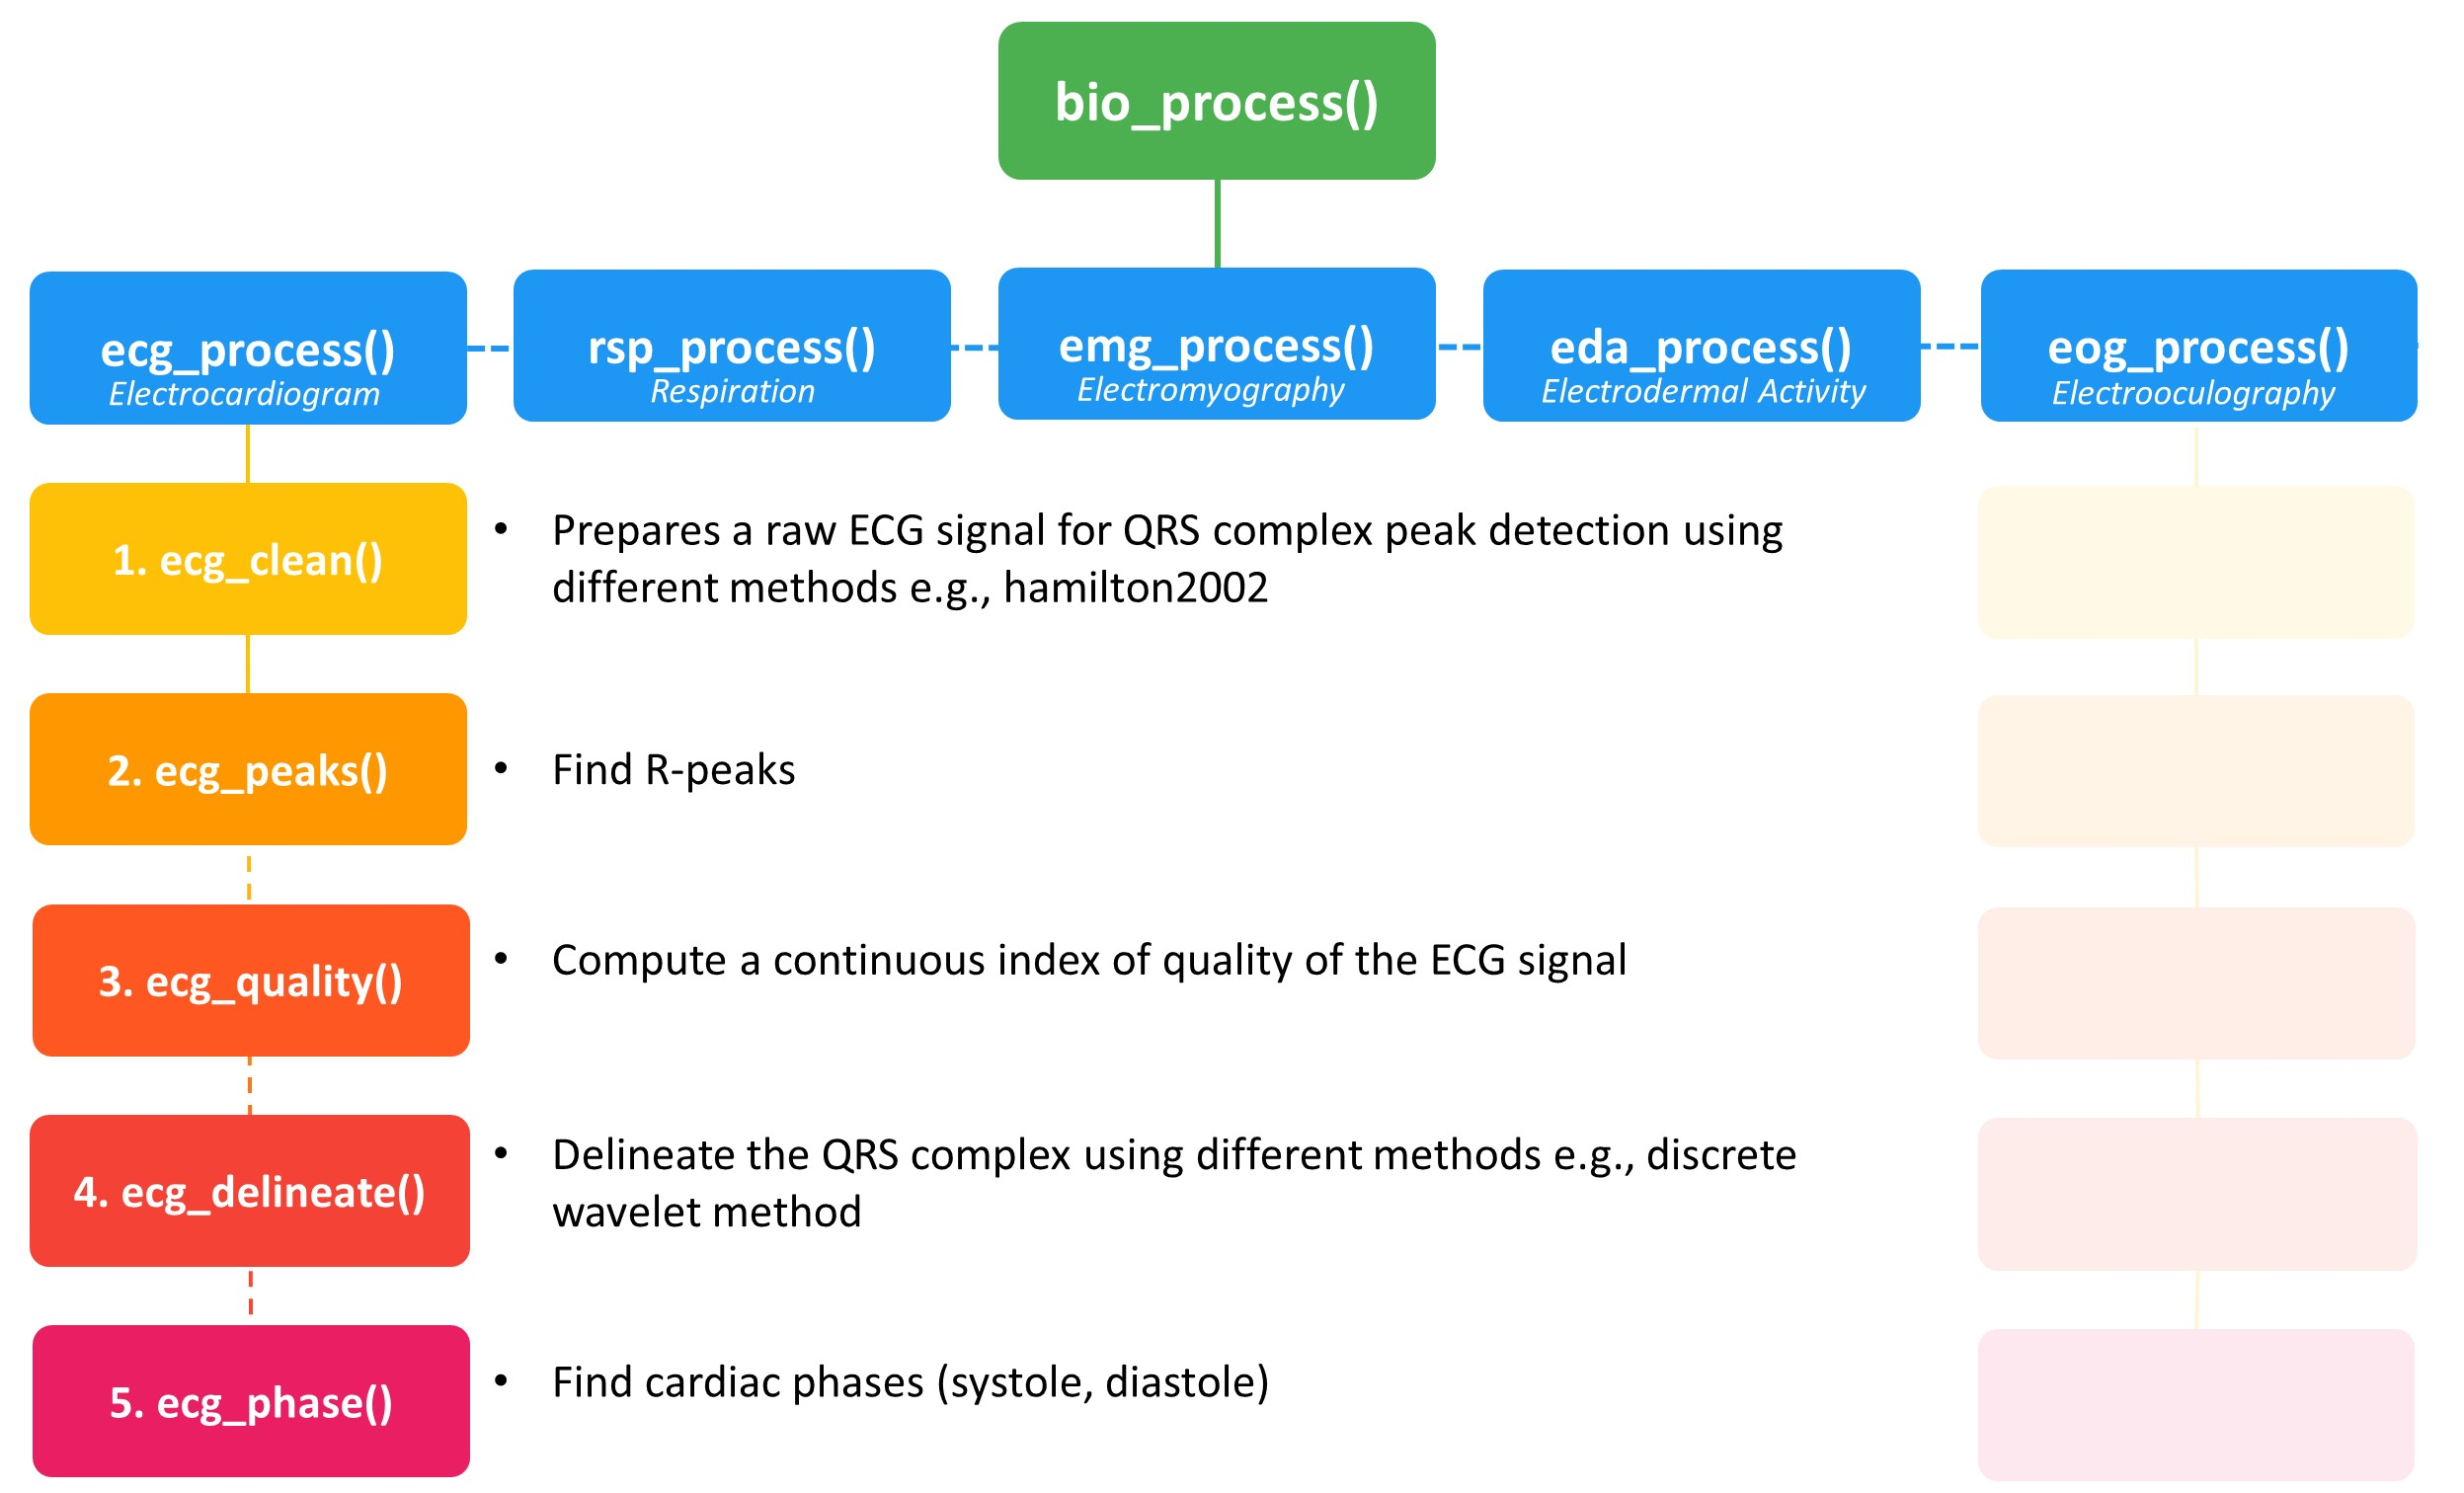
\includegraphics[width=1\linewidth]{figures/nk_architecture} \caption{Illustration of the NeuroKit2 package architecture, in the case of ECG signal processing.}\label{fig:unnamed-chunk-1}
\end{figure}

The mid-level functions are assembled in high-level wrappers, that are convenient entry points for new users. For instance, the \texttt{ecg\_process()} function internally chains the mid-level functions \texttt{ecg\_clean()}, \texttt{ecg\_peaks()}, \texttt{ecg\_quality()}, \texttt{ecg\_delineate()}, and \texttt{ecg\_phase()}, as shown in \textbf{Figure 1}. A specific processing pipeline can be selected with the \texttt{method} argument that is then propagated throughout the internal functions. Easily switching between processing pipelines allows for the comparison of different methods, and streamlines critical but time-consuming steps in reproducible research, such as the validation of data preparation and quality control (Quintana, Alvares, \& Heathers, 2016). Finally, the package includes convenience-functions (e.g., \texttt{bio\_process}) that enable the combined processing of multiple types of signals at once (e.g., \texttt{bio\_process(ecg=ecg\_signal,\ eda=eda\_signal)}).

Performing an entire set of operations with sensible default parameters in one function can be rewarding, especially for beginners, allowing them to perform cutting-edge processing or replication of research steps without requiring much programming expertise. Moreover, it contributes to the demystification of the usage of programming tools (as opposed to GUI-based software such as \emph{SPSS}, \emph{Kubios}, or \emph{Acqknowledge}), providing a welcoming framework to further explore physiological data processing. Importantly, more advanced users can build custom analysis pipelines by using the low- and mid-level functions, allowing for finer control over the processing parameters. We believe that this implementation is a well-calibrated trade-off between flexibility and user-friendliness.

\hypertarget{installing-neurokit2}{%
\section{Installing NeuroKit2}\label{installing-neurokit2}}

\emph{NeuroKit2} is available on PyPI, a repository of software for the Python programming language. and can be installed using pip (via \enquote{\emph{pip install neurokit2}} command). Detailed instructions on how to install Python are also available in the \emph{installation} section of the package's documentation.

\hypertarget{examples}{%
\section{Examples}\label{examples}}

In this section, we present two examples that illustrate the most common use-cases. Both examples can be accessed in an interactive format (without any prior installation) via a \emph{\href{https://mybinder.org/v2/gh/neuropsychology/NeuroKit/master?urlpath=lab\%2Ftree\%2Fdocs\%2Fexamples}{Binder environment}}.The first example illustrates an interval-related paradigm where characteristics of physiological activity during a certain time interval (not necessarily tied to a specific and sudden event) are extracted. The second example presents an event-related paradigm, in which the interest lies in shorter-term physiological changes related to specific events (see \textbf{Figure 1} and \textbf{Table 1}). The example datasets are available with the package and can be downloaded using the \texttt{data()} function. This utility reads comma separated values files (\emph{.csv}) with the Pandas function \emph{pd.read\_csv()}, where each column is a different biosignal. Each row is a sample that correspond to signals' value at a given point in time. All examples use the 0.0.41 version release of \emph{NeuroKit2}.

\textbackslash begin\{figure\}
\includegraphics[width=1\linewidth]{figures/features} \textbackslash caption\{Plot window displaying a period of raw electrocardiogram (ECG in red), respiration (RSP in blue) and electrodermal activity (EDA in purple) data. The green highlighted section, spanning from 0 to 20s, represents the periodic region of interest during interval-related analysis. The 3 event markers are indicated by dotted lines, and the orange highlighted sections spanning 0.1s before the onset of each event and ending 4s after the event, represent periodic regions of interest during event-related analysis. The link for generating the figure can be found on NeuroKit2's GitHub repository (\url{https://github.com/neuropsychology/NeuroKit/blob/master/paper/make_figures.Rmd})\}\label{fig:unnamed-chunk-2}
\textbackslash end\{figure\}

\begin{table}[!h]

\caption{\label{tab:table3pdf}Examples of features computed in different domains.}
\centering
\fontsize{9}{11}\selectfont
\begin{tabular}[t]{>{\raggedright\arraybackslash}p{8cm}>{\raggedright\arraybackslash}p{8cm}}
\toprule
Interval-related Features & Event-related Features\\
\midrule
ECG Rate Characteristics (Mean, Amplitude) & ECG Rate Changes (Min, Mean, Max, Time of Min,  Max, Trend)\\
Heart Rate Variability (HRV) indices & RSP Rate Changes (Min, Mean, Max, Time of Min, Max)\\
Respiratory Rate Variability (RRV) indices & RSP Amplitude Measures (Min, Mean, Max)\\
Respiratory Sinus Arrhythmia (RSA) indices & ECG and RSP Phase (Inspiration/Expiration, Systole/Diastole, Completion)\\
Number of SCR Peaks and mean amplitude & SCR peak and its characteristics (amplitude, rise time, recovery time)\\
\bottomrule
\end{tabular}
\end{table}

\hypertarget{interval-related-paradigm}{%
\subsection{Interval-related Paradigm}\label{interval-related-paradigm}}

The first dataset corresponds to 5 minutes of physiological activity of a human participant at rest (eyes-closed in a seated position), with no specific instructions. It contains three channels (ECG, PPG and RSP) sampled at a frequency of 100Hz.

\begin{Shaded}
\begin{Highlighting}[]
\CommentTok{# Load the package}
\ImportTok{import}\NormalTok{ neurokit2 }\ImportTok{as}\NormalTok{ nk}

\CommentTok{# Download the example dataset}
\NormalTok{data }\OperatorTok{=}\NormalTok{ nk.data(}\StringTok{"bio_resting_5min_100hz"}\NormalTok{)}

\CommentTok{# Process the data}
\NormalTok{df, info }\OperatorTok{=}\NormalTok{ nk.bio_process(ecg}\OperatorTok{=}\NormalTok{data[}\StringTok{"ECG"}\NormalTok{],}
\NormalTok{                          rsp}\OperatorTok{=}\NormalTok{data[}\StringTok{"RSP"}\NormalTok{],}
\NormalTok{                          sampling_rate}\OperatorTok{=}\DecValTok{100}\NormalTok{)}

\CommentTok{# Extract features}
\NormalTok{results }\OperatorTok{=}\NormalTok{ nk.bio_analyze(df, sampling_rate}\OperatorTok{=}\DecValTok{100}\NormalTok{)}

\CommentTok{# Show subset of results}
\NormalTok{results[[}\StringTok{"ECG_Rate_Mean"}\NormalTok{, }\StringTok{"HRV_RMSSD"}\NormalTok{, }\StringTok{"RSP_Rate_Mean"}\NormalTok{, }\StringTok{"RSA_P2T_Mean"}\NormalTok{]]}
\end{Highlighting}
\end{Shaded}

\begin{table}[!h]

\caption{\label{tab:table2pdf}Subset of properties characterizing the physiological activity over a period of 5 minutes of resting-state.}
\centering
\begin{tabular}[t]{rrrr}
\toprule
ECG\_Rate\_Mean & HRV\_RMSSD & RSP\_Rate\_Mean & RSA\_P2T\_Mean\\
\midrule
86.39 & 38.84 & 15.74 & 0.07\\
\bottomrule
\end{tabular}
\end{table}

Here, the aim was to illustrate a type of physiological analysis that we refer to as interval-related (or resting-state paradigm, as opposed to an event-related paradigm). After loading the package and the example dataset, each physiological signal is processed using \texttt{bio\_process()}.
As we want to compute features related to the entire dataset (see \textbf{Table 2}), we can directly pass the whole dataframe to \texttt{bio\_analyze()}, and compute the interval-related features. Users can choose a specific time interval from their dataset.

Interval-related analyses compute features of signal variability and activation patterns over a given period of time, including average heart and breathing rate, as well as indices of heart rate variability (HRV) and respiratory sinus arrhythmia (RSA). \emph{NeuroKit2} allows for the fast creation of standardized and reproducible pipelines to describe this kind of physiological activity.

\hypertarget{event-related-paradigm}{%
\subsection{Event-related Paradigm}\label{event-related-paradigm}}

This example dataset contains ECG, RSP and EDA signals of one participant who was presented with four emotional images (from the NAPS database; Marchewka, Żurawski, Jednoróg, \& Grabowska, 2014) in a typical (albeit shortened) experimental psychology paradigm.

The signals are 2.5 minutes (150 seconds) long and are recorded at a frequency of 100Hz (note that the sampling rate is lower than usually required, see Quintana et al., 2016, in order to be able to include the example data in the \emph{NeuroKit2} distribution). It has 4 channels including three physiological signals, and one corresponding to events marked with a photosensor (signal strength decreases when a stimulus appears on the screen).

\begin{Shaded}
\begin{Highlighting}[]
\CommentTok{# Load the package}
\ImportTok{import}\NormalTok{ neurokit2 }\ImportTok{as}\NormalTok{ nk}

\CommentTok{# Download the example dataset}
\NormalTok{data }\OperatorTok{=}\NormalTok{ nk.data(}\StringTok{"bio_eventrelated_100hz"}\NormalTok{)}

\CommentTok{# Process the data}
\NormalTok{df, info }\OperatorTok{=}\NormalTok{ nk.bio_process(ecg}\OperatorTok{=}\NormalTok{data[}\StringTok{"ECG"}\NormalTok{],}
\NormalTok{                          rsp}\OperatorTok{=}\NormalTok{data[}\StringTok{"RSP"}\NormalTok{],}
\NormalTok{                          eda}\OperatorTok{=}\NormalTok{data[}\StringTok{"EDA"}\NormalTok{],}
\NormalTok{                          sampling_rate}\OperatorTok{=}\DecValTok{100}\NormalTok{)}

\CommentTok{# Find events}
\NormalTok{conditions }\OperatorTok{=}\NormalTok{ [}\StringTok{"Negative"}\NormalTok{, }\StringTok{"Neutral"}\NormalTok{, }\StringTok{"Neutral"}\NormalTok{, }\StringTok{"Negative"}\NormalTok{]}
\NormalTok{events }\OperatorTok{=}\NormalTok{ nk.events_find(event_channel}\OperatorTok{=}\NormalTok{data[}\StringTok{"Photosensor"}\NormalTok{],}
\NormalTok{                        threshold_keep}\OperatorTok{=}\StringTok{'below'}\NormalTok{,}
\NormalTok{                        event_conditions}\OperatorTok{=}\NormalTok{conditions)}

\CommentTok{# Epoch the data}
\NormalTok{epochs }\OperatorTok{=}\NormalTok{ nk.epochs_create(data}\OperatorTok{=}\NormalTok{df,}
\NormalTok{                          events}\OperatorTok{=}\NormalTok{events,}
\NormalTok{                          sampling_rate}\OperatorTok{=}\DecValTok{100}\NormalTok{,}
\NormalTok{                          epochs_start}\OperatorTok{=-}\FloatTok{0.1}\NormalTok{,}
\NormalTok{                          epochs_end}\OperatorTok{=}\DecValTok{4}\NormalTok{)}

\CommentTok{# Extract event related features}
\NormalTok{results }\OperatorTok{=}\NormalTok{ nk.bio_analyze(epochs, sampling_rate}\OperatorTok{=}\DecValTok{100}\NormalTok{)}

\CommentTok{# Show subset of results}
\NormalTok{results[[}\StringTok{"Condition"}\NormalTok{, }\StringTok{"ECG_Rate_Mean"}\NormalTok{, }\StringTok{"RSP_Rate_Mean"}\NormalTok{, }\StringTok{"EDA_Peak_Amplitude"}\NormalTok{]]}
\end{Highlighting}
\end{Shaded}

\begin{table}[!h]

\caption{\label{tab:table1pdf}Subset of the ouput related to event-related analysis characterizing the pattern of physiological changes related to specific stimuli.}
\centering
\begin{tabular}[t]{lrrr}
\toprule
Condition & ECG\_Rate\_Mean & RSP\_Rate\_Mean & EDA\_Peak\_Amplitude\\
\midrule
Negative & -2.01 & -0.15 & 0.93\\
Neutral & -3.13 & 1.40 & 0.41\\
Neutral & 1.34 & -0.34 & 0.02\\
Negative & -3.55 & 1.97 & 1.06\\
\bottomrule
\end{tabular}
\end{table}

In this example, the steps of the analysis are identical to the previous example, including loading the package, the dataset and processing the data. The difference is that stimulus onsets in the photosensor are detected separately with \texttt{events\_find()}. Once we have the preprocessed signals and the location of events, we use \texttt{epochs\_create()} to slice the data into segments corresponding to a time window (ranging from -0.1 to 4 seconds) around each stimulus. Finally, relevant features are computed for each epoch (i.e., each stimulus) by passing them to \texttt{bio\_analyze()}.

Notably, the features include the changes in rate of ECG and RSP signals (e.g.~maximum, minimum and mean rate after stimulus onset, and the time at which they occur), and the peak characteristics of the EDA signal (e.g., occurrence of skin conductance response (SCR), and if SCR is present, its corresponding peak amplitude, time of peak, rise and recovery time). In addition, respiration and cardiac cycle phases are extracted (i.e., the respiration phase - inspiration/expiration - and cardiac phase - systole/diastole - occurring at the onset of event).

We hope that these examples demonstrate how straightforward the process of extracting features of physiological responses can be with \emph{NeuroKit2}. This pipeline can easily scale up to group-level analyses by aggregating the average of features across participants. In addition to streamlining data analyses, \emph{NeuroKit2} aims to allow researchers to extract an extensive suite of features that can be linked to neurocognitive processes. In this example (see \textbf{Table 3}), exposure to negative stimuli, as compared to neutral stimuli, is related to stronger cardiac deceleration, higher skin conductance response, and accelerated breathing rate (note that this descriptive interpretation is given solely for illustrative purposes).

\hypertarget{discussion}{%
\section{Discussion}\label{discussion}}

\emph{NeuroKit2} is a neurophysiological signal processing library accessible to people across different levels of programming experience and backgrounds. For users who are novice programmers or are new to neurophysiology, the package presents an ideal opportunity for exploration and learning. The experienced programmer is encouraged to choose and validate the preprocessing and analysis pipelines most appropriate for their data. Suggestions for improvements or additions to the library are welcome and openly discussed in the community. Overall, the development of \emph{NeuroKit2} is focused on creating an intuitive user-experience, as well as building a collaborative community. Its modular structure and organization not only facilitate the use of existing and validated processing pipelines, but also create a fertile ground for experimentation and innovation.

The library is also a pragmatic answer to the broader need for transparent and reproducible methods in neurophysiology. The impact of our package on reproducibility in research is two-fold: firstly, while black-box software can be easy and convenient to use, users do not have access to the source code, making processing results subject to unknown idiosyncrasies of the underlying implementation of processing routines. This makes it difficult to identify the source of potential discrepancies in results obtained with other software and can lead to irreproducible findings. In contrast, \emph{NeuroKit2} documents each step of the implementation along with the analysis method, allowing users to pin-point the analysis steps where differences might arise. While maintaining a focus on overall user-experience, the open-source nature of \emph{NeuroKit2} encourages independent researchers to cross-validate research findings. Secondly, not only does \emph{NeuroKit2} implement several methods for analysis, it also allows for the comparison of different algorithms. For instance, using a suite of open-source databases, different algorithms for ECG R-peak detection have been compared for their robustness (number of errors encountered), efficiency (computation time) and accuracy (absolute distance from true R-peak location), documented in the \enquote{Studies} section of the package's documentation. As \emph{NeuroKit2} continues to work on benchmarking, we hope to support users in making more informed decisions regarding which method is most suited for their specific requirements.

\emph{NeuroKit2} also prioritizes a high standard of quality control during code development. This is done through automated testing using continuous integration, as well as striving for code simplicity and readability. The API is thoroughly documented, including working examples. We ensure that the documentation evolves alongside the code by including it in our continuous integration. While \emph{NeuroKit2} currently has a fairly comprehensive documentation, more examples and tutorials will be added as the package grows and expands. Additionally, we provide thorough guidelines for new contributors who wish to contribute code or documentation.

We expect the package's future evolution to be driven by the communities' needs and the advances in related fields. For instance, although \emph{NeuroKit2} already implements a lot of useful functions for EEG processing (such as entropy and fractal dimensions quantification), its support could be further improved (for example with high-level functions built on top of utilities provided by the leading EEG Python software, namely \emph{MNE}; Gramfort et al., 2013). Additionally, in the future we strive to support other types of bodily signals (e.g., electrogastrography - EGG, electrooculography - EOG) and plan to optimize computational efficiency on large datasets. We also plan to further validate the available processing pipelines using public databases. In line with this objective, the support of standardized data structure formats (e.g.~WFDB, BIDS, \ldots) could be extended.

In conclusion, we believe that \emph{NeuroKit2} provides useful tools for anyone who is interested in analyzing physiological data collected with research-grade hardware or wearable \enquote{smart health devices}. By increasing the autonomy of researchers and practitioners, and by shortening the delay between data collection and results acquisition, \emph{NeuroKit2} could be useful beyond academic research in neuroscience and psychology, including applications such as personal physiological monitoring and exercise science. Finally, we hope that \emph{NeuroKit2} encourages users to become part of a supportive open-science community with diverse areas of expertise rather than relying on closed-source and proprietary software, thus shaping the future of neurophysiology and its related fields.

\hypertarget{conflict-of-interest}{%
\section{Conflict of Interest}\label{conflict-of-interest}}

The authors declare that the research was conducted in the absence of commercial or financial relationships that could constitute a conflict of interest.

\hypertarget{acknowledgements}{%
\section{Acknowledgements}\label{acknowledgements}}

We would like to thank Prof.~C. F. Xavier for inspiration, all the current and future contributors (\url{https://neurokit2.readthedocs.io/en/latest/authors.html}), and the users for their support. Additionally, François Lespinasse would like to thank the Courtois Foundation for its support through the Courtois-NeuroMod project (\url{https://cneuromod.ca})

\newpage

\hypertarget{references}{%
\section{References}\label{references}}

\begingroup
\setlength{\parindent}{-0.5in}
\setlength{\leftskip}{0.5in}

\hypertarget{refs}{}
\leavevmode\hypertarget{ref-bach2014head}{}%
Bach, D. R. (2014). A head-to-head comparison of scralyze and ledalab, two model-based methods for skin conductance analysis. \emph{Biological Psychology}, \emph{103}, 63--68.

\leavevmode\hypertarget{ref-HRV}{}%
Bartels, R., \& Pecanha, T. (2020). HRV: A pythonic package for heart rate variability analysis. \emph{Journal of Open Source Software}, \emph{5}(51), 1867. \url{https://doi.org/10.21105/joss.01867}

\leavevmode\hypertarget{ref-benedek2010continuous}{}%
Benedek, M., \& Kaernbach, C. (2010). A continuous measure of phasic electrodermal activity. \emph{Journal of Neuroscience Methods}, \emph{190}(1), 80--91.

\leavevmode\hypertarget{ref-biosppy}{}%
Carreiras, C., Alves, A. P., Lourenço, A., Canento, F., Silva, H., Fred, A., \& others. (2015). \emph{BioSPPy: Biosignal processing in Python}. Retrieved from \url{https://github.com/PIA-Group/BioSPPy/}

\leavevmode\hypertarget{ref-clifton2012machine}{}%
Clifton, D. A., Gibbons, J., Davies, J., \& Tarassenko, L. (2012). Machine learning and software engineering in health informatics. \emph{2012 first international workshop on realizing ai synergies in software engineering (raise)}, 37--41. IEEE.

\leavevmode\hypertarget{ref-PySiology}{}%
Gabrieli, G., Azhari, A., \& Esposito, G. (2019). PySiology: A python package for physiological feature extraction. In \emph{Neural approaches to dynamics of signal exchanges} (pp. 395--402). Springer Singapore. \url{https://doi.org/10.1007/978-981-13-8950-4_35}

\leavevmode\hypertarget{ref-HeartPy}{}%
Gent, P. van, Farah, H., Nes, N. van, \& Arem, B. van. (2019). HeartPy: A novel heart rate algorithm for the analysis of noisy signals. \emph{Transportation Research Part F: Traffic Psychology and Behaviour}, \emph{66}, 368--378. \url{https://doi.org/10.1016/j.trf.2019.09.015}

\leavevmode\hypertarget{ref-gomes2019pyhrv}{}%
Gomes, P., Margaritoff, P., \& Silva, H. (2019). PyHRV: Development and evaluation of an open-source python toolbox for heart rate variability (hrv). \emph{Proc. Int'l conf. On electrical, electronic and computing engineering (icetran)}, 822--828.

\leavevmode\hypertarget{ref-gramfort2013meg}{}%
Gramfort, A., Luessi, M., Larson, E., Engemann, D. A., Strohmeier, D., Brodbeck, C., \ldots{} others. (2013). MEG and eeg data analysis with mne-python. \emph{Frontiers in Neuroscience}, \emph{7}, 267.

\leavevmode\hypertarget{ref-greco2015cvxeda}{}%
Greco, A., Valenza, G., Lanata, A., Scilingo, E. P., \& Citi, L. (2015). CvxEDA: A convex optimization approach to electrodermal activity processing. \emph{IEEE Transactions on Biomedical Engineering}, \emph{63}(4), 797--804.

\leavevmode\hypertarget{ref-harris2020array}{}%
Harris, C. R., Millman, K. J., Walt, S. J. van der, Gommers, R., Virtanen, P., Cournapeau, D., \ldots{} others. (2020). Array programming with numpy. \emph{Nature}, \emph{585}(7825), 357--362.

\leavevmode\hypertarget{ref-matplotlib}{}%
Hunter, J. D. (2007). Matplotlib: A 2D graphics environment. \emph{Computing in Science \& Engineering}, \emph{9}(3), 90--95.

\leavevmode\hypertarget{ref-Jupyter2018}{}%
Jupyter, Bussonnier, Forde, Freeman, Granger, Head, \ldots{} Willing. (2018). Binder 2.0 - Reproducible, interactive, sharable environments for science at scale. In Fatih Akici, David Lippa, Dillon Niederhut, \& M. Pacer (Eds.), \emph{Proceedings of the 17th Python in Science Conference} (pp. 113--120). \url{https://doi.org/\%2010.25080/Majora-4af1f417-011\%20}

\leavevmode\hypertarget{ref-khodadad2018optimized}{}%
Khodadad, D., Nordebo, S., Mueller, B., Waldmann, A., Yerworth, R., Becher, T., \ldots{} others. (2018). Optimized breath detection algorithm in electrical impedance tomography. \emph{Physiological Measurement}, \emph{39}(9), 094001.

\leavevmode\hypertarget{ref-Kiverstein2015}{}%
Kiverstein, J., \& Miller, M. (2015). The embodied brain: Towards a radical embodied cognitive neuroscience. \emph{Frontiers in Human Neuroscience}, \emph{9}, 237.

\leavevmode\hypertarget{ref-kluyver2016jupyter}{}%
Kluyver, T., Ragan-Kelley, B., Pérez, F., Granger, B. E., Bussonnier, M., Frederic, J., \ldots{} others. (2016). Jupyter notebooks-a publishing format for reproducible computational workflows. \emph{ELPUB}, 87--90.

\leavevmode\hypertarget{ref-Systole}{}%
Legrand, N., \& Allen, M. (2020). \emph{Systole: A python toolbox for preprocessing, analyzing, and synchronizing cardiac data}. Retrieved from \url{https://github.com/embodied-computation-group/systole}

\leavevmode\hypertarget{ref-maizey2019barriers}{}%
Maizey, L., \& Tzavella, L. (2019). Barriers and solutions for early career researchers in tackling the reproducibility crisis in cognitive neuroscience. \emph{Cortex}, \emph{113}, 357--359.

\leavevmode\hypertarget{ref-neurokit1}{}%
Makowski, D. (2020). Neurokit: A python toolbox for statistics and neurophysiological signal processing (eeg, eda, ecg, emg...). Retrieved from \url{https://github.com/neuropsychology/NeuroKit.py}

\leavevmode\hypertarget{ref-marchewka2014nencki}{}%
Marchewka, A., Żurawski, Ł., Jednoróg, K., \& Grabowska, A. (2014). The nencki affective picture system (naps): Introduction to a novel, standardized, wide-range, high-quality, realistic picture database. \emph{Behavior Research Methods}, \emph{46}(2), 596--610.

\leavevmode\hypertarget{ref-pandas}{}%
McKinney, W., \& others. (2010). Data structures for statistical computing in python. \emph{Proceedings of the 9th python in science conference}, \emph{445}, 51--56. Austin, TX.

\leavevmode\hypertarget{ref-milkowski2018replicability}{}%
Miłkowski, M., Hensel, W. M., \& Hohol, M. (2018). Replicability or reproducibility? On the replication crisis in computational neuroscience and sharing only relevant detail. \emph{Journal of Computational Neuroscience}, \emph{45}(3), 163--172.

\leavevmode\hypertarget{ref-open2015estimating}{}%
Nosek, B. A., Cohoon, J., Kidwell, M., \& Spies, J. R. (2015). Estimating the reproducibility of psychological science. \emph{Science}, \emph{349}(6251), aac4716.

\leavevmode\hypertarget{ref-scikit-learn}{}%
Pedregosa, F., Varoquaux, G., Gramfort, A., Michel, V., Thirion, B., Grisel, O., \ldots{} Duchesnay, E. (2011). Scikit-learn: Machine learning in Python. \emph{Journal of Machine Learning Research}, \emph{12}, 2825--2830.

\leavevmode\hypertarget{ref-Quintana2016}{}%
Quintana, D., Alvares, G. A., \& Heathers, J. (2016). Guidelines for reporting articles on psychiatry and heart rate variability (graph): Recommendations to advance research communication. \emph{Translational Psychiatry}, \emph{6}(5), e803--e803.

\leavevmode\hypertarget{ref-roy2019deep}{}%
Roy, Y., Banville, H., Albuquerque, I., Gramfort, A., Falk, T. H., \& Faubert, J. (2019). Deep learning-based electroencephalography analysis: A systematic review. \emph{Journal of Neural Engineering}, \emph{16}(5), 051001.

\leavevmode\hypertarget{ref-nolds}{}%
Schölzel, C. (2019). \emph{Nonlinear measures for dynamical systems}. Zenodo. \url{https://doi.org/10.5281/zenodo.3814723}

\leavevmode\hypertarget{ref-tarvainen2014kubios}{}%
Tarvainen, M. P., Niskanen, J.-P., Lipponen, J. A., Ranta-Aho, P. O., \& Karjalainen, P. A. (2014). Kubios hrv--heart rate variability analysis software. \emph{Computer Methods and Programs in Biomedicine}, \emph{113}(1), 210--220.

\leavevmode\hypertarget{ref-topalidou2015long}{}%
Topalidou, M., Leblois, A., Boraud, T., \& Rougier, N. P. (2015). A long journey into reproducible computational neuroscience. \emph{Frontiers in Computational Neuroscience}, \emph{9}, 30.

\leavevmode\hypertarget{ref-python3}{}%
Van Rossum, G., \& Drake, F. L. (2009). \emph{Python 3 reference manual}. Scotts Valley, CA: CreateSpace.

\leavevmode\hypertarget{ref-scipy}{}%
Virtanen, P., Gommers, R., Oliphant, T. E., Haberland, M., Reddy, T., Cournapeau, D., \ldots{} Contributors, S. 1. 0. (2020). SciPy 1.0: Fundamental Algorithms for Scientific Computing in Python. \emph{Nature Methods}, \emph{17}, 261--272. \url{https://doi.org/https://doi.org/10.1038/s41592-019-0686-2}

\leavevmode\hypertarget{ref-yuehong2016internet}{}%
Yuehong, Y., Zeng, Y., Chen, X., \& Fan, Y. (2016). The internet of things in healthcare: An overview. \emph{Journal of Industrial Information Integration}, \emph{1}, 3--13.

\endgroup


\end{document}
